\section{Hearing}

\subsection{Range of human hearing}
\bi

\i The frequency range of human hearing is roughly
20~Hz to 20~kHz.
This is a factor of $1000$ or roughly 10 octaves
($2^{10} = 1024$) in frequency.

\i The pressure variation range of human hearing at 1000~Hz is
roughly $2\times 10^{-5}~{\rm Pa}$ (threshold of hearing)
to $20~{\rm Pa}$ (threshold of pain).
This is a factor of $10^6$ in pressure variation or $10^{12}$
in intensity (${\rm Watt/m}^2$).

\i Compared to standard atmospheric pressure $P_{\rm atm} = 100~{\rm kPa}$,
these values are only $2\times 10^{-10}$ and
$2\times 10^{-4}$ of atmospheric pressure, respectively.
So even at the threshold of pain, the pressure change is only a few 
parts in $10^4$ of atmospheric pressure!

\i In contrast, the frequency range for human vision is
only a factor of 2 (so 1 octave);
and the intensity range of human vision is only a factor of
$10^5$ (versus $10^{12}$ for human hearing).
Thus, the human ear is a much more sensitive device than the
human eye!

\ei
%%%%%%%%%%%%%%%%%%%%%%%%%%%%%%%%%%%%%%%%%%%%%%%%
\subsection{Fechner's law}
\bi

\i G.~T. Fechner in ``Elements of psychophysics" ($\sim 1860$):
``As stimuli are increased by multiplication, sensation
increases by addition."

\i In later sections we'll see that Fechner's law 
applies
{\em approximately} to our perceptions of both the 
pitch and loudness of a sound.
(Fechner's law applies to other sensations as well, 
such as sight and smell.)

\i Mathematically, Fechner's law means that sensation is 
proportional to the {\em logarithm} of a stimulus.

\i Recall the defintion of the logarithm:%
%
\be
y = \log x
\quad
\Leftrightarrow
\quad
x = 10^y
\ee
%

\i Some useful values to remember:
%
\be
\log 2 \approx 0.3\,,\quad
\log 3 \approx 0.5\,,\quad
\log 4 \approx 0.6\,,\quad
\log 5 \approx 0.7\,,\quad
\log 10 = 1
\ee
%

\i Logarithms allow us to compress a large dynamic range 
of a stimulus to a much smaller (i.e., manageable) range.
This was probably advantageous to us from an evolutionary
perspective.

\ei
%%%%%%%%%%%%%%%%%%%%%%%%%%%%%%%%%%%%%%%%%%%%%%%%
\subsection{The human ear}
\bi

\i The human auditory system consists of two parts: 
(i) the peripheral auditory system made up of the ear, and
(ii) the central auditory system made of the brain and the
auditory nervous system.

\i The human ear can be divided functionally into 
three basic parts
(the outer, middle, and inner ear) as shown in 
Figure~\ref{f:human-ear-diagram}.
%
\begin{figure}[htbp]
\begin{center}
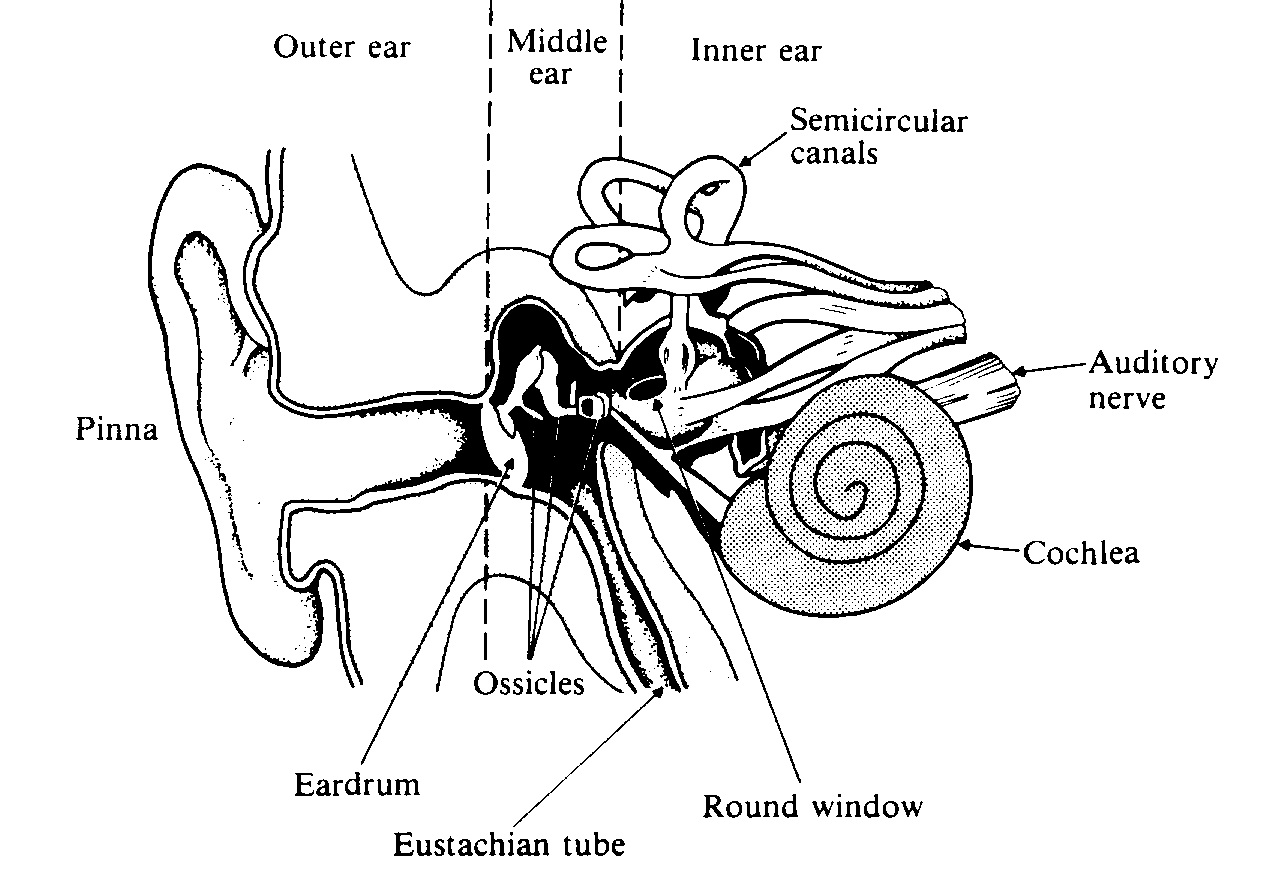
\includegraphics[width=.8\textwidth]{human-ear-diagram.jpg}
\caption{A drawing of the human ear, showing the division into
the outer, middle, and inner ear.  
Note that this drawing is not to scale.
(From ``Science of Sound" by Rossing, Moore, and Wheeler.)}
\label{f:human-ear-diagram}
\end{center}
\end{figure}
%

\i The outer ear consists of the pinna and auditory canal,
which collects the sound (i.e., pressure waves in the air)
and funnels it to the middle ear.

\i The middle ear consists of the ear drum and ossicles
(three small bones called the hammer, anvil, and stirrup,
based on their shapes).
The pressure wave at the ear drum is amplified ($\sim 30\times$) 
by the ossicles as it is transmitted to the oval window.
 
\i The inner ear consists of the semi-circular canals,
which are responsible for balance, and the 
cochlea, which is responsible for converting the mechanical
sound waves to electrical impulses that get sent to the
brain via the auditory nerve.

\i A schematic representation of the ear is shown in
Figure~\ref{f:human-ear-schematic}.
%
\begin{figure}[htbp]
\begin{center}
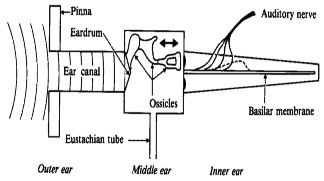
\includegraphics[width=.8\textwidth]{human-ear-schematic.jpg}
\caption{A schematic representation of the human ear, with an
uncoiled cochlea.
(From ``Science of Sound" by Rossing, Moore, and Wheeler.)}
\label{f:human-ear-schematic}
\end{center}
\end{figure}
%

\i In Figure~\ref{f:human-ear-schematic}, the cochlea is unwound.
The length of an unwound cochlea is approximately 3.5~cm (so a 
little less than 1.5~inches).
The basilar membrane divides the cochlear tube into two sections
called the {\em scala vestibuli} at the top of the diagram, 
and the {\em scala tympani} at the bottom.
The ossicle bones are, from left to right, 
the hammer, anvil, and stirrup.

\i Figure~\ref{f:cochlea-uncoiled} is a schematic
representation of an unwound cochlea.
%
\begin{figure}[htbp]
\begin{center}
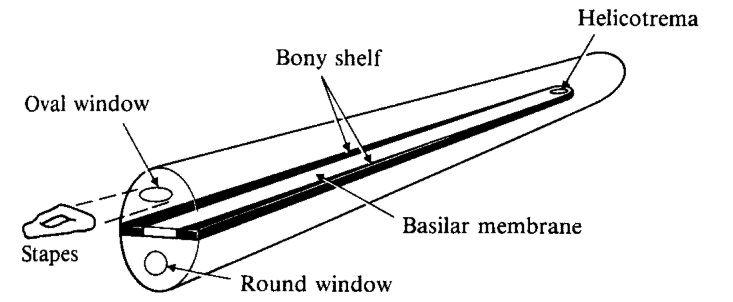
\includegraphics[width=.8\textwidth]{cochlea-uncoiled.jpg}
\caption{A schematic representation of an unwound cochlea.
The region above the basilar membrane is called the {\em scala vestibuli};
the region below the basilar membrane is called the {\em scala tympani}.
The helicotrema is a hole in the basilar membrane connecting
the two sections of the cochlea. 
(From ``Science of Sound" by Rossing, Moore, and Wheeler.)}
\label{f:cochlea-uncoiled}
\end{center}
\end{figure}
%

\i The organ of Corti rests on the basilar membrane.
It contains rows of tiny hair cells that are connected to
the auditory nerve fibers.

\i Each hair cells has many hairs, called {\em stereocilia},
which bend in response to motions of the basilar membrane.
The bending of the stereocilia stimulate the hair cells,
which trigger the auditory nerve fibers to send electrical
impulses to the brain.

\i When the stapes (stirrups) press against the oval window,
a pressure wave is set up in the cochlear fluid, causing
the basilar membrane to have ripples as shown in 
Figure~\ref{f:cochlea-uncoiled-schematic}.
%
\begin{figure}[htbp]
\begin{center}

\includegraphics[width=.8\textwidth]{cochlea-uncoiled-schematic.png}
\caption{A schematic representation showing the effects of
a pressure wave propagating through the cochlear fluid.
OW stands for oval window; RW for round window;
SV for scala vestibuli; ST for scala tympani; and
H for helicotrema.
The location of maximum displacement of the basilar membrane
(BM) depends on the frequency of the sound.
(From {\tt commons.wikimedia.org}.)}
\label{f:cochlea-uncoiled-schematic}
\end{center}
\end{figure}
%

\i The location of maximum displacement of the basilar 
membrane depends on the frequency of the incident sound wave:
{\em High-frequency} sound waves produce maximum displacements 
of the basilar membrane {\em closer} to the stirrups;
{low-frequency} sound waves produce maximum displacements 
of the basilar membrane {\em further} from the stirrups.

\i A pure tone (i.e., a single frequency sound wave)
excites a relatively wide region (1.3~mm, having 
approximately 1300~neurons) of the basilar membrane.
This region is called a {\em critical band}.

\i There are 24 critical bands on the basilar membrane
that span the audible frequency range from $20$ to $\approx 20~$kHz.

\i The center frequencies of the critical bands are spaced 
logarithmically along the basilar membrane, similar to 
the frequencies of the keys on a piano keyboard.
In other words, equal distances along the basilar membrane 
correspond to equal ratios of the central frequencies as shown
in Figure~\ref{f:basilar-resonance-max}.
%
\begin{figure}[htbp]
\begin{center}
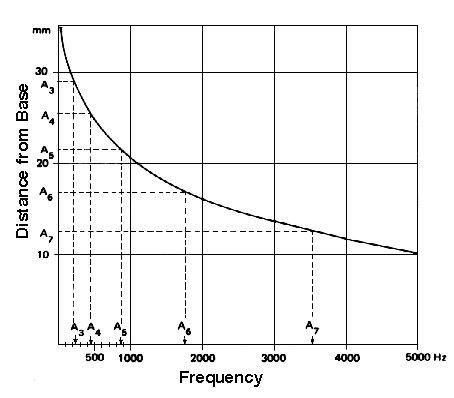
\includegraphics[width=.6\textwidth]{basilar-resonance-max.jpg}
\caption{Position of the maximum displacement on 
the basilar membrane as a function of the pure tone 
frequency.
(From ``Science of Sound" by Rossing, Moore, and Wheeler.)}
\label{f:basilar-resonance-max}
\end{center}
\end{figure}
%

\i Thus, the location of maximum displacement of the 
basilar membrane has a {\em logarithmic frequency response},
in agreement with Fechner's law.

\i The bandwidths of the critical bands are approximately
constant ($\approx 100$~Hz) for frequencies below about 500~Hz;
at higher frequencies, the bandwidths increase in proportion 
to the center frequencies, having values approximately equal
to one-fourth of an octave (so 3 semitones or approximately
15\%) about each center frequency.

\i The fact that the human ear acts like a spectrum analyser 
for sound waves (with different parts of the basilar membrane
repsonding to different frequency sound waves) 
is called the {\em place theory of pitch}.

\i Sound waves can enter the inner ear via {\em air conduction} 
as discussed above.
They can also enter the inner ear via {\em bone conduction} through 
the skull.

\i Humming is an example of a sound that is heard mostly 
via bone conduction.
By plugging your ears with your fingers when humming 
(thus blocking the air path), the humming can actually sound louder.

\i Hearing through bone conduction is the reason why our
voices sound different when we hear ourselves speak on a tape recorder.
The microphone of a tape recorder picks up our voice as it 
is heard via air conduction.
But we hear our own voice partly via air conduction and partly via
bone conduction.

\ei
%%%%%%%%%%%%%%%%%%%%%%%%%%%%%%%%%%%%%%%%%%%%%%%
\subsection{Binaural hearing and sound localization}
\bi

\i The fact that we have two ears allows us to better 
locate the source of a sound (similar to depth perception
using two eyes---i.e., binocular vision).
 
\i For frequencies above about 4000~Hz, localization is
accomplished via an {\em intensity} difference of the 
sound reaching the two ears.
At these higher frequencies, sound does not easily 
diffract around the head, so one ear is effectively in
the ``shadow" of the head and receives less intense sound.
The brain interprets the ear that hears the less 
intense sound as being further from the source of sound.

\i For frequencies below about 1000~Hz, localization is
accomplished via a difference in the {\em time of arrival}
(or, equivalently, a phase difference) of the sound 
reaching the two ears.
The brain interprets the ear that hears the time-delayed 
sound as being further from the source of the sound.

\ei
